\begin{figure}[t!]
    \centering
    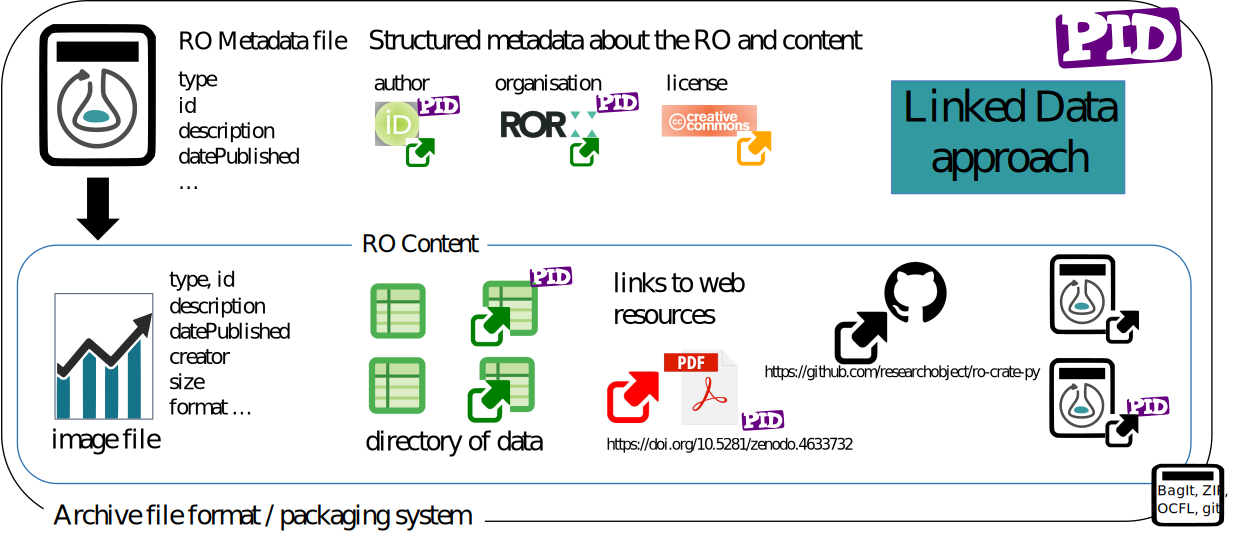
\includegraphics[width=0.95\textwidth]{content/images/ro-crate-overview.pdf}
\caption{\textbf{Conceptual overview of RO-Crate}. A \emph{Persistent Identifier} (PID) \cite{doi:10.1371/journal.pbio.2001414} points to a \emph{Research Object} (RO), which may be archived using different packaging approaches like BagIt \cite{doi:10.17487/rfc8493}, OCFL \cite{ocfl_2020}, git or ZIP. The RO is described within a \emph{RO-Crate Metadata File}, providing identifiers for \emph{authors} using ORCID, \emph{organisations} using Research Organization Registry (ROR) \cite{doi:10.6087/kcse.192} and licences such as Creative Commons using SPDX identifiers. The \emph{RO-Crate content} is further described with additional metadata following a Linked Data approach. Data can be embedded files and directories, as well as links to external Web resources, PIDs and nested RO-Crates.}
    \label{fig:conceptual}
\end{figure}
